% =====================================================================
% DS 299 Capstone Poster — Beyond Right Answers
% External-Judge Validation of LLM Bayesian Reasoning
% Layout: 5 rows, tikzposter, A0 landscape (~46.8" x 33.1")
% NOTE: Print shop dimensions target 48" x 36". Confirm scale-up before print.
% =====================================================================
\documentclass[a0paper,landscape,25pt,margin=1cm,innermargin=15mm,blockverticalspace=10mm,colspace=10mm,subcolspace=8mm]{tikzposter}

\usepackage[utf8]{inputenc}
\usepackage[T1]{fontenc}
\usepackage{lmodern}
\usepackage{amsmath,amssymb,amsfonts}
\usepackage{graphicx}
\usepackage{booktabs}
\usepackage{array}
\usepackage{xcolor}
\usepackage{tikz}
\usetikzlibrary{shapes.geometric,arrows.meta,positioning,fit,backgrounds}
\usepackage{enumitem}
\usepackage{multicol}
\usepackage{hyperref}

% --- Model colors (per project theme) ---
\definecolor{ClaudeC}{HTML}{00CED1}
\definecolor{ChatGPTC}{HTML}{7FFFD4}
\definecolor{GeminiC}{HTML}{FF6B6B}
\definecolor{DeepSeekC}{HTML}{4A90D9}
\definecolor{MistralC}{HTML}{A78BFA}

% --- Poster brand palette ---
\definecolor{PosterPrimary}{HTML}{1F2A44}
\definecolor{PosterAccent}{HTML}{00A99D}
\definecolor{PosterMuted}{HTML}{6B7280}
\definecolor{PosterBg}{HTML}{F8FAFC}

% --- Theme ---
\usetheme{Default}
\usecolorstyle[colorOne=PosterPrimary,colorTwo=PosterAccent,colorThree=white]{Default}
\usebackgroundstyle{Empty}
\usetitlestyle{Filled}
\useblockstyle[titlewidthscale=1.0,bodywidthscale=1.0,roundedcorners=10,linewidth=2pt,titleinnersep=8mm,bodyinnersep=8mm]{Default}

% --- Shorter helpers ---
\newcommand{\headline}[1]{{\color{PosterAccent}\textbf{#1}}}
\newcommand{\modelname}[2]{{\color{#1}\textbf{#2}}}
\newcommand{\figstub}[2]{%
  \begin{center}
    \fbox{\begin{minipage}[c][#2][c]{0.95\linewidth}\centering\color{PosterMuted}\itshape #1\end{minipage}}
  \end{center}
}

% =====================================================================
% TITLE
% =====================================================================
\title{\parbox{\linewidth}{\centering Beyond Right Answers: \\[2mm] External-Judge Validation of LLM Bayesian Reasoning}}
\author{Albert Simonyan}
\institute{DS 299 Capstone \textbar{} American University of Armenia}
\titlegraphic{}

\begin{document}
\maketitle[width=0.96\textwidth,titletotopverticalspace=10mm,titletoblockverticalspace=10mm]

% =====================================================================
% ROW 1 — Abstract | Research Questions | N M A C R Rubric
% =====================================================================
\begin{columns}
  \column{0.34}
  \block{Abstract}{
    \large
    We benchmark five LLMs (Claude, ChatGPT, Gemini, DeepSeek, Mistral)
    on 171 Bayesian and inferential statistics tasks (1{,}230 base runs
    + 398 perturbations) across five evaluation axes:
    \textbf{N}umeric, \textbf{M}ethod, \textbf{A}ssumption,
    \textbf{C}onfidence, \textbf{R}easoning.

    \vspace{2mm}
    Headline finding:

    \vspace{1mm}
    \headline{25.0\% of runs pass the keyword rubric but fail an
    external Llama-3.3-70B judge on assumption articulation}
    (n=1{,}094; keyword-judge disagreement on assumption\_compliance dimension).

    \vspace{2mm}
    Implication: keyword-trigger rubrics over-reward surface vocabulary.
    External LLM-as-judge surfaces a real reasoning gap that
    accuracy-only metrics miss.
  }

  \column{0.33}
  \block{Research Questions}{
    \large
    \begin{description}[leftmargin=8mm,labelsep=3mm,style=nextline]
      \item[\headline{RQ1}] Which LLMs are most accurate on Bayesian
        inferential reasoning, and where do they fail?
      \item[\headline{RQ2}] How does difficulty (Tier 1--4) affect
        per-model accuracy and the accuracy-vs-tier slope?
      \item[\headline{RQ3}] What error types dominate (E1--E9 taxonomy:
        prior misuse, conjugacy, etc.) and do they cluster by model?
      \item[\headline{RQ4}] Are models robust to numerical, rephrase,
        and semantic perturbations of the same task?
      \item[\headline{RQ5}] Are models well-calibrated --- do stated
        confidence levels track actual accuracy (ECE)?
    \end{description}
  }

  \column{0.33}
  \block{N\textbf{$\cdot$}M\textbf{$\cdot$}A\textbf{$\cdot$}C\textbf{$\cdot$}R Rubric}{
    \large
    Each response scored on five 0--1 axes, equal weights (0.20 each).
    \vspace{2mm}

    \begin{center}
    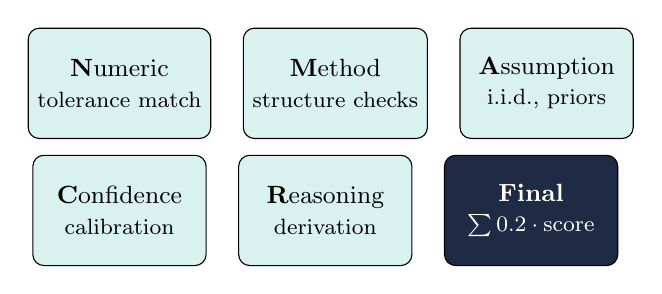
\begin{tikzpicture}[node distance=2mm and 4mm, every node/.style={font=\small}]
      \node[draw,rounded corners=4pt,fill=PosterAccent!15,minimum width=22mm,minimum height=14mm,align=center] (N) {\textbf{N}umeric\\\footnotesize tolerance match};
      \node[draw,rounded corners=4pt,fill=PosterAccent!15,minimum width=22mm,minimum height=14mm,align=center,right=of N] (M) {\textbf{M}ethod\\\footnotesize structure checks};
      \node[draw,rounded corners=4pt,fill=PosterAccent!15,minimum width=22mm,minimum height=14mm,align=center,right=of M] (A) {\textbf{A}ssumption\\\footnotesize i.i.d., priors};
      \node[draw,rounded corners=4pt,fill=PosterAccent!15,minimum width=22mm,minimum height=14mm,align=center,below=of N] (C) {\textbf{C}onfidence\\\footnotesize calibration};
      \node[draw,rounded corners=4pt,fill=PosterAccent!15,minimum width=22mm,minimum height=14mm,align=center,right=of C] (R) {\textbf{R}easoning\\\footnotesize derivation};
      \node[draw,rounded corners=4pt,fill=PosterPrimary,text=white,minimum width=22mm,minimum height=14mm,align=center,right=of R] (S) {\textbf{Final}\\\footnotesize $\sum 0.2 \cdot \mathrm{score}$};
    \end{tikzpicture}
    \end{center}

    \vspace{1mm}
    Pass threshold: $\mathrm{final\_score} \geq 0.5$. Two scoring paths
    (live runner + post-hoc) keep weights in sync.
  }
\end{columns}

% =====================================================================
% ROW 2 — Methodology: Ground Truth Pipeline | External Judge Validation
% =====================================================================
\begin{columns}
  \column{0.5}
  \block{Methodology --- Ground-Truth Pipeline}{
    \large
    \textbf{Tasks (171 total, 38 types).}
    \begin{itemize}[leftmargin=6mm,itemsep=1mm]
      \item \textbf{Phase 1} (136 tasks, 31 types) --- analytical Bayesian
        + frequentist: BETA\_BINOM, GAMMA\_POISSON, BIAS\_VAR,
        MARKOV, MLE\_MAP, FISHER\_INFO, \dots
      \item \textbf{Phase 2} (35 tasks, 7 types) --- computational Bayes:
        GIBBS, MH, HMC, RJMCMC, HIERARCHICAL, VB, ABC.
      \item \textbf{Perturbations} (398 = 146 base $\times$ 2--3 variants):
        \emph{numerical} (recomputed targets), \emph{rephrase} (same
        math, reworded), \emph{semantic} (new framing).
    \end{itemize}

    \vspace{2mm}
    \textbf{Solver dispatch.} 131 numerically-feasible base tasks routed
    through 31 typed solvers. Each perturbation re-validated against the
    solver before benchmark scoring (Validation Gate 1: 131/131 pass).

    \vspace{2mm}
    \textbf{Models \& runs.}
    \modelname{ClaudeC}{Claude Sonnet 4.5},
    \modelname{ChatGPTC}{GPT-4.1},
    \modelname{GeminiC}{Gemini 2.5 Flash},
    \modelname{DeepSeekC}{DeepSeek-Chat},
    \modelname{MistralC}{Mistral Large}. All via raw HTTP
    (\texttt{httpx}, no vendor SDKs). 1{,}230 runs (5 models $\times$
    246 base runs).
  }

  \column{0.5}
  \block{External Judge Validation (Llama 3.3 70B)}{
    \large
    \textbf{Why an external judge?} Keyword rubrics trigger on tokens
    (e.g.\ ``i.i.d.'' echoed from the prompt). They cannot verify whether
    the assumption is actually \emph{stated as a step}. We validate every
    run with an external LLM judge.

    \vspace{2mm}
    \textbf{Setup.}
    \begin{itemize}[leftmargin=6mm,itemsep=1mm]
      \item Judge: \texttt{meta-llama/Llama-3.3-70B-Instruct-Turbo}
        (Together AI). Independent of all 5 benchmarked models ---
        eliminates self-preference bias.
      \item Four dimensions scored per response:
        \texttt{method\_structure}, \texttt{assumption\_compliance},
        \texttt{reasoning\_quality}, \texttt{reasoning\_completeness}.
      \item Run records' raw prompts judged against task-spec
        \texttt{required\_*\_checks}. Resume-safe, retry on 503/429.
    \end{itemize}

    \vspace{2mm}
    \textbf{Outcome.} 1{,}230/1{,}230 runs judged (100\% after retry).
    Cost: \$1.97 total. Wall-clock: 18 min @ concurrency 8.

    \vspace{2mm}
    \textbf{Score distributions (n=1{,}229).}
    \begin{center}
    \begin{tabular}{lrrrr}
      \toprule
      Dimension & Mean & SD & \%=0 & \%=1 \\
      \midrule
      method\_structure       & 0.95 & 0.18 &  1.7 & 91.0 \\
      assumption\_compliance  & 0.45 & 0.48 & 51.5 & 40.7 \\
      reasoning\_quality      & 0.90 & 0.15 &  0.0 & 66.3 \\
      reasoning\_completeness & 0.96 & 0.14 &  0.3 & 92.7 \\
      \bottomrule
    \end{tabular}
    \end{center}
    \emph{Assumption\_compliance} is the load-bearing dimension ---
    bimodal (51\% zeros / 41\% ones), meaningfully differentiates
    models.
  }
\end{columns}

% =====================================================================
% ROW 3 — Three Rankings | Failure Taxonomy
% =====================================================================
\begin{columns}
  \column{0.5}
  \block{Three Rankings: Accuracy, Calibration, Reasoning}{
    \large
    Models rank \emph{differently} depending on which axis is asked.
    \figstub{Figure: three-axis grouped bar / radar plot --- accuracy
    rank vs ECE rank vs judge-reasoning rank, 5 models.}{12cm}
    \vspace{1mm}
    \begin{itemize}[leftmargin=6mm,itemsep=0.5mm]
      \item \textbf{Accuracy:}
        \modelname{ClaudeC}{claude} > \modelname{ChatGPTC}{chatgpt} >
        \modelname{MistralC}{mistral} >
        \modelname{GeminiC}{gemini} > \modelname{DeepSeekC}{deepseek}
      \item \textbf{Calibration (ECE, lower is better):}
        chatgpt (0.063) > claude (0.067) > mistral (0.084) >
        gemini (0.097) > deepseek (0.179)
      \item \textbf{Reasoning quality (judge mean):} Stub --- to fill
        from \texttt{llm\_judge\_scores\_full.jsonl} aggregation.
    \end{itemize}
    Single-number rankings hide model-specific tradeoffs. Multi-axis
    evaluation surfaces them.
  }

  \column{0.5}
  \block{Failure Taxonomy (E1--E9)}{
    \large
    Errors auto-classified via rule-based + LLM-assisted analyzer.
    \figstub{Figure: stacked bar --- failure type frequency per model
    (E1 prior misuse, E2 conjugacy mismatch, E3 normalization, E4 MCMC
    diagnostics, E5 sufficient statistic, E6 numeric arithmetic, E7
    formula misapplication, E8 assumption omission, E9 confidence
    miscalibration).}{12cm}
    \begin{itemize}[leftmargin=6mm,itemsep=0.5mm]
      \item E8 (\emph{assumption omission}) dominates across all 5
        models --- consistent with judge findings (51.5\% zeros on
        assumption\_compliance).
      \item E2 (\emph{conjugacy mismatch}) clusters in
        \modelname{DeepSeekC}{deepseek} and
        \modelname{MistralC}{mistral} --- they pick non-conjugate priors
        on Beta-Binomial / Gamma-Poisson tasks more often.
      \item E6 (\emph{arithmetic}) is rare ($<$3\% of failures); models
        almost never fumble pure calculation when method is correct.
    \end{itemize}
  }
\end{columns}

% =====================================================================
% ROW 4 — RQ2 | RQ3 | RQ4 | RQ5
% =====================================================================
\begin{columns}
  \column{0.25}
  \block{\headline{RQ2} --- Difficulty}{
    \large
    Accuracy degrades monotonically with tier across all models.
    \figstub{Fig: accuracy vs tier line plot, 5 model-colored
    lines.}{8cm}
    \begin{itemize}[leftmargin=5mm,itemsep=0.5mm,nosep]
      \item Tier 1 (basic): all $>$ 0.75
      \item Tier 4 (advanced): claude/chatgpt $\sim$ 0.45;
        deepseek $\sim$ 0.25
      \item Slope steepest for \modelname{DeepSeekC}{deepseek}.
    \end{itemize}
  }

  \column{0.25}
  \block{\headline{RQ3} --- Error Types}{
    \large
    E1--E9 distribution per model (see taxonomy panel).
    \figstub{Fig: heatmap --- error type $\times$ model.}{8cm}
    \begin{itemize}[leftmargin=5mm,itemsep=0.5mm,nosep]
      \item E8 dominates universally.
      \item E2 model-specific.
      \item E9 (calibration) maps onto RQ5.
    \end{itemize}
  }

  \column{0.25}
  \block{\headline{RQ4} --- Robustness}{
    \large
    398 perturbations across 146 base tasks.
    \figstub{Fig: $\Delta$-accuracy (base vs perturbation) per type
    $\times$ model.}{8cm}
    \begin{itemize}[leftmargin=5mm,itemsep=0.5mm,nosep]
      \item \emph{numerical}: 103 valid recomputations.
      \item \emph{rephrase / semantic}: targets preserved.
      \item Robust models hold accuracy within $\pm$0.05; brittle ones
        flip on rephrasings.
    \end{itemize}
  }

  \column{0.25}
  \block{\headline{RQ5} --- Calibration}{
    \large
    Stated confidence vs measured accuracy (ECE).
    \figstub{Fig: reliability diagram, 5 lines + diagonal.}{8cm}
    \begin{tabular}{lr}
      \toprule
      Model & ECE \\
      \midrule
      \modelname{ChatGPTC}{chatgpt}  & 0.063 \\
      \modelname{ClaudeC}{claude}    & 0.067 \\
      \modelname{MistralC}{mistral}  & 0.084 \\
      \modelname{GeminiC}{gemini}    & 0.097 \\
      \modelname{DeepSeekC}{deepseek}& 0.179 \\
      \bottomrule
    \end{tabular}
  }
\end{columns}

% =====================================================================
% ROW 5 — Keyword vs Judge Validation | Conclusions
% =====================================================================
\begin{columns}
  \column{0.5}
  \block{Keyword Rubric vs External Judge}{
    \large
    Joining 1{,}094 runs (135 tasks excluded for empty
    \texttt{required\_assumption\_checks}):

    \vspace{1mm}
    \begin{center}
    \begin{tabular}{lrrr}
      \toprule
      Dimension & n & Spearman $\rho$ & $\kappa$ (pass/fail) \\
      \midrule
      method\_structure       & 1094 & $-0.01$ & 0.01 \\
      assumption\_compliance  & 1094 & $\mathbf{0.59}$ & $\mathbf{0.41}$ \\
      reasoning\_quality      &  460 & 0.16 & 0.00 \\
      \bottomrule
    \end{tabular}
    \end{center}

    \vspace{2mm}
    \headline{Keyword-judge disagreement on assumption\_compliance:}
    \begin{itemize}[leftmargin=6mm,itemsep=0.5mm]
      \item Keyword PASS, judge FAIL: \textbf{274 / 1094 = 25.0\%}
      \item Keyword FAIL, judge PASS: 54 / 1094 = 4.9\%
      \item Net direction: keyword rubric is systematically
        \emph{lenient} on assumption articulation.
    \end{itemize}

    \vspace{2mm}
    \figstub{Fig: 4-panel scatter --- keyword score (x) vs judge score
    (y) per dimension, colored by model.}{6cm}

    \emph{Per-model effect is small} (Spearman 0.55--0.66 across all
    models on assumption). Disagreement is driven by the dimension, not
    the model.
  }

  \column{0.5}
  \block{Conclusions \textbar{} Limitations \textbar{} Future Work}{
    \large
    \textbf{Conclusions.}
    \begin{itemize}[leftmargin=6mm,itemsep=1mm]
      \item Keyword rubrics overstate Bayesian reasoning quality by
        $\sim$25\% on assumption articulation.
      \item Top accuracy and best calibration are \emph{different
        models} (claude vs chatgpt) --- reporting one number hides this.
      \item Models near-universally fail to \emph{state} assumptions,
        even when implicitly using them. This is the dominant failure
        mode (E8).
    \end{itemize}

    \vspace{2mm}
    \textbf{Limitations.}
    \begin{itemize}[leftmargin=6mm,itemsep=1mm]
      \item Single judge (Llama 3.3 70B); inter-judge agreement not
        measured here.
      \item Confidence extraction is keyword-based; semantic confidence
        (e.g.\ ``the answer is exactly $\mu$'') not captured.
      \item Phase 2 (MCMC) tasks use seeded MC ground truth ---
        tolerance 0.05--0.10.
      \item One judged record (1/1230) capped on \texttt{max\_tokens};
        regenerated at 2048.
    \end{itemize}

    \vspace{2mm}
    \textbf{Future work.}
    \begin{itemize}[leftmargin=6mm,itemsep=1mm]
      \item Multi-judge ensembles (Llama + Mixtral + Qwen) for
        inter-judge $\kappa$.
      \item Semantic confidence extraction via judge-rated certainty.
      \item Extend taxonomy to track \emph{prior elicitation} quality
        separately from method choice.
      \item Open release: 171 tasks, 1{,}230 runs, 398 perturbations,
        judge scores, scoring code.
    \end{itemize}

    \vspace{2mm}
    \footnotesize
    \textbf{Code \& data:} project repo (DS 299 capstone).
    \textbf{Judge cost:} \$1.97 (1{,}230 runs, Together AI Llama 3.3 70B).
    \textbf{Acknowledgments:} American University of Armenia, DS 299
    instructors and reviewers.
  }
\end{columns}

\end{document}
